\section{Choice of pre-period and controls}
\label{sec:design}
The target is the average effect of a replication report on citations to the papers assessed, separately by its source-coded outcome. For report cohort $g$, outcome label $s$, and event time $k$, the target is
\[
 \operatorname{ATT}_{s}(g,k)
 = E\!\left[Y_{i,g+k}(g)-Y_{i,g+k}(\infty)
       \mid G_i=g,\ S_i=s,\ i\in\mathcal{S}\right].
\]
Here $\mathcal{S}$ is the set of completed comparisons under the stated matching specification. The corresponding target over all eligible originals would require completed collection or additional assumptions about selection into this subset. The reported three-year response averages $k=1,2,3$, then averages over originals with equal weight. $Y(g)$ is the citation path with a report at $g$ and $Y(\infty)$ the path without that report. Cohort aggregation should weight original papers equally. The difference between outcome-specific ATTs describes different groups of papers; it is not the effect of assigning a failed rather than successful outcome. The implemented matched contrasts estimate these targets only under the identifying assumptions in the main text.

\subsection{Retain long histories; separate matching from measurement}
We retain citation histories from indexed publication through \CitationsThrough{}. The primary specification uses five complete pre-report years to choose controls, while measuring change between the last three pre-report years and the first three post-report years. The outcome contrast stays fixed when the matching history changes. Three-year matching is a sensitivity; eight- and ten-year matching examine older originals.

Table~\ref{tab:history} separates availability from age. Longer baselines exclude papers assessed soon after publication even if collection is complete. Five years retains \FiveHistoryN{} comparisons; eight and ten retain \EightHistoryN{} and \TenHistoryN{}. We selected five years after inspecting these coverage counts and before inspecting the longer-history effect estimates. The original three-year estimates had already been examined. This is an exploratory design revision, not a preregistration.

\begin{table}[H]
\centering
\caption{Availability of longer matching histories.}
\label{tab:history}
\small
\begin{tabular}{lrrrr}
\toprule
Matching years & Old enough & Available & Common sample & Missing baseline \\
\midrule
3 & 961 & 282 & 82 & 477 \\
5 & 729 & 227 & 82 & 338 \\
8 & 385 & 109 & 82 & 186 \\
10 & 278 & 82 & 82 & 131 \\
\bottomrule
\end{tabular}

\par\smallskip\begin{minipage}{\linewidth}\footnotesize
The starting roster has \EligibleOriginals{} eligible originals. Old enough applies only the original's publication-age condition, not follow-up or controls. Available additionally requires a complete pool, baseline histories, and selected follow-up. Missing baseline counts otherwise feasible comparisons blocked by uncollected baseline histories. The same \CommonHistoryN{} originals support every matching length. Columns overlap and are not additive exclusions.
\end{minipage}
\end{table}

The available-sample comparison mixes changes in matching and paper composition. Figure~\ref{fig:history} therefore also holds the originals fixed. Every point uses three years before and three after to measure the outcome; only the matching-history specification changes. Eligible and selected controls can still change. Older citations reveal persistent differences, but distant history need not predict current citation growth well. Longer matching is not automatically better matching.

\begin{figure}[H]
\centering
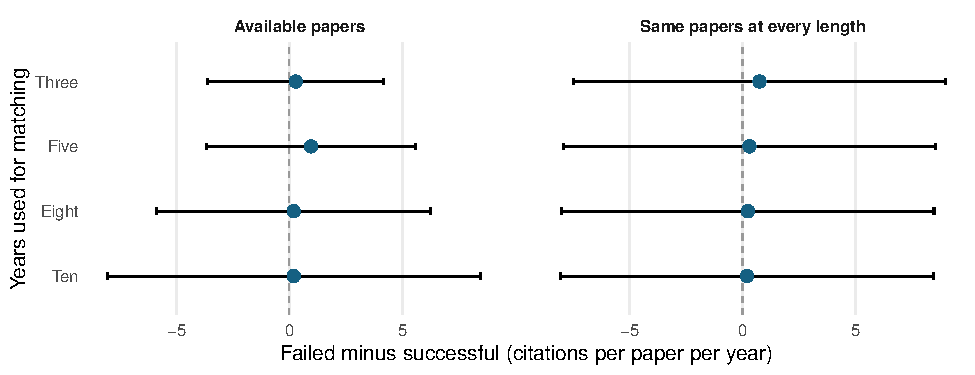
\includegraphics[width=\linewidth]{matching_history.pdf}
\caption{Sensitivity to matching-history length. Points show failed-minus-successful matched changes; bars are 95\% paper/report clustered intervals conditional on matches. The left panel uses available papers at each length; the right uses the same \CommonHistoryN{} originals, with controls reselected. Panels share an axis and outcome window: the last three pre-report years versus the first three post-report years.}
\label{fig:history}
\end{figure}

Pre-fit can look good because it was optimized. We therefore select controls using the earlier years of each five-, eight-, or ten-year history and reserve the final two pre-report years for validation. The five-year check fits on years minus five through minus three and evaluates years minus two and minus one. No post-report citation count enters selection. Table~\ref{tab:validation} reports the held-out level gap and difference in changes. Unlike the older pre-window diagnostic in Table~\ref{tab:diagnostics}, this exercise trains new matches and evaluates later pre-period observations. Both condition on the completed-comparison sample. Neither is independent confirmation or proof of parallel trends; early disclosure could contaminate the final pre-report years. We do not select papers by whether a pre-trend test rejects.

\begin{table}[H]
\centering
\caption{Prediction of pre-report citations outside the matching period.}
\label{tab:validation}
\small
\begin{tabular}{llrrr}
\toprule
History & Outcome & Originals & Level gap & Change gap \\
\midrule
5 years & Failed & 112 & $+8.53$ & $+1.56$ \\
5 years & Successful & 115 & $+18.55$ & $+0.66$ \\
8 years & Failed & 50 & $+13.65$ & $+0.04$ \\
8 years & Successful & 59 & $+30.73$ & $-0.59$ \\
10 years & Failed & 39 & $+15.24$ & $+0.56$ \\
10 years & Successful & 43 & $+41.17$ & $-0.93$ \\
\bottomrule
\end{tabular}

\par\smallskip\begin{minipage}{\linewidth}\footnotesize
Controls are reselected without the last two pre-report years. The level gap is the original-minus-control mean over those years. The change gap is the original-minus-control difference in the one-year change between them. Units are annual citations per paper. These descriptive diagnostics have no inferential intervals and condition on the available sample at each history length.
\end{minipage}
\end{table}

\subsection{Define the pool before choosing the nearest papers}
The preferred pool is the full set of research papers of the same indexed publication year, journal, and article type as each original. This holds publication age and venue approximately fixed and subjects controls to the same calendar years. Publisher dates establish that papers existed before the baseline. The present random sample of twenty candidates is a computational shortcut, not the definition of an appropriate counterfactual. The next collection should enumerate the full pool, acquire histories, and then select controls. Adding history cannot recover a close match omitted from the pool.

Assessed and unassessed papers can differ in visibility, topic, and expected replicability. Matching must be evaluated on prior citation levels and changes. Topic restrictions based on the original published text are a possible sensitivity; later citations, later journal impact, and responses to the replication are inappropriate matching variables. For expanded pools, we propose an overlap restriction: the original must lie inside the pool's annual citation range in every matching year. Report excluded originals separately and compare this restricted population with the unrestricted pool. This coordinate-wise rule does not guarantee a close joint trajectory, so held-out prediction errors still matter. Freeze any additional distance caliper using pre-period prediction before estimating post-period contrasts in the expanded sample.

If the full same-journal/year pool lacks support, report that limitation. A separate alternative can broaden publication year within the journal or use field/year peers in other journals, but requires adjustment for publication age or venue. We should not widen the pool until a preferred post-report answer appears.

The current implementation excludes every known assessed paper and papers currently marked retracted. The preferred longitudinal pool instead records dated replication, reproduction, and retraction events. A control must be unexposed at the focal report date and contributes only through years before its own exposure. A conservative sensitivity uses controls unassessed throughout the outcome window. Current retraction flags and exclusion of every eventual assessment condition eligibility on events after some focal reports. Those retrospective exclusions remain in this snapshot; dated risk-set construction and full-pool collection are not completed analyses.

\subsection{Estimation and causal interpretation}
The primary estimator is a matched difference in differences, with separate averages for successful and failed outcomes and equal weight per original. An unmatched same-journal/year comparison should accompany expanded collection so the consequences of matching are visible. Neither matching nor fixed effects establishes parallel trends.

With dated exposures and larger pools, a cohort-specific event study can estimate each lead and lag and aggregate with explicit original-paper weights. Group-time estimators allow never-assessed or not-yet-assessed controls without using already assessed papers as untreated comparisons \citep{callaway2021}. Cohort-interacted event studies are another established option \citep{sun2021}. A pooled two-way fixed-effects regression that uses earlier-treated papers as controls for later-treated papers is not proposed. The current within-comparison change estimator does not make those comparisons.

Synthetic difference in differences is a secondary candidate for cohorts with long, balanced histories and enough controls \citep{arkhangelsky2021}. Standard synthetic DiD fits unit weights using pre-treatment trajectories and time weights using control outcomes before and after treatment. Pre-period placebo exercises can assess the procedure without using treated post-period outcomes to choose it. Its block-treatment implementation requires common onset within each fitted cohort. Concatenating staggered reports as simultaneous would change the design. Good fit and placebo ranks would not establish random assignment.

The event should ultimately be the earliest verified public release of an assessment, with journal publication analyzed separately. Where first disclosure cannot be established, the journal-date analysis must remain labeled accordingly. Later reports and author responses should be dated, with censoring treated as a change in the estimand.

Causal interpretation requires credible untreated comparisons, no anticipation, and no differential shocks to citation growth. Topic-wide attention and selection of unusually visible papers for replication are plausible violations. The held-out gaps and poor level matches give reasons for caution. Completing pools, dating exposures, and reporting longer paths are prerequisites for stronger interpretation, not guarantees of it. Inference should retain dependence from reused papers and shared reports; current intervals condition on matches and labels and exclude uncertainty about disclosure dates and design selection.
